\Chapter{Gesztusok}

\Section{Felismerendő gesztusok}

A szoftver használata közben a prezentáló személy különféle gesztusok segítségével irányíthatja a prezentáció menetét és szintén ezen gesztusok segítségével léphet kapcsolatba a videófolyamon megjelenő virtuális elemekkel. A felhasználó a karjai segítségével valósíthatja meg a mozdulatokat. A gesztusokat az alábbi kategóriákba sorolhatjuk:

\begin{itemize}
\item \textbf{Sweep}: Egyenes vonalú mozgás. A mozgásnak van iránya és két képkocka között megfigyelhető a hossza is.
\item \textbf{Shift}: Bizonyos virtuális elemek közvetlenül is reagálnak a környezetükben történő mozgásra. Az ilyen elemek az irányukba történő mozgással megegyező irányú mozgással reagálnak. Vagyis a prezentáló személy például a kezei segítségével egyszerűen eltolhatja az adott virtuális elemet.
\item \textbf{Blink}: Az ujjak gyors ökölbe zárása vagy a tenyér széttárásának mozdulata.
\item \textbf{Drag}: Bizonyos virtuális elemeket a prezentáló személy képes megfogni, majd odébbhúzni és elengedni. A funkció eléréséhez a prezentálónak egy \textit{Blink} gesztust kell végrehajtania. Az elkapás pillanatában az adott objektum a \textit{Blink} pozíciójára (a prezentáló kézfejére) tapad és követi annak helyzetét. A felhasználó így tetszőleges irányba mozgathatja az "elkapott" elemet. Egy újabb \textit{Blink} gesztussal pedig a kívánt helyére teheti azt.
\item \textbf{Rotation}: A videófolyamon történő örvénylő mozgás, ami akár több ponton is megfigyelhető. Ez lehet például karlendítés, körvonal/ív menti mozgás, tenyerek forgatása.
\item \textbf{Többpontos kezelés}: A képen lévő összefüggő, nagyobb elmozdulások keresése, \textit{Blob}-ok alapján. Több pont egymáshoz képesti vizsgálata különféle szempontok alapján.
\end{itemize}

\Section{Képek és vektor mezők}

Az elmozdulás becslésére az ún. \textit{Motion-Flow} technikák tűntek a legalkalmasabbnak. Egy kiemelkedő és széles körben elterjedt eljárás a Bruce D. Lucas és Takeo Kanade által kidolgozott módszer, melynek implementálása az \textit{OpenCV}-ben is megtalálható.

A Lucas-Kanade módszer dedikált pontok követésére hivatott. Ha a videófomlyaból kiemelünk két képkockát, melyek között az eltelt idő kicsi, a módszer képes megbecsülni a két képkockán elhelyezkedő kijelölt pontok pozíciójának a változását, vagyis megadja a pontok elmozdulás vektorát. A módszer azon a megállapításon alapszik, hogy a videófolyamon egy kijelölt pont és a körülötte lévő pixelek halmaza közel azonos intenzitású $(I)$ a vizsgált időintervallumban. Ha a ponthoz tartozó valós objektum elmozdul a korábbi helyzetéről és az általa képviselt új pont a vizsgálandó pont bizonyos tartományába esik, akkor a módszer képes becslést adni a pont új helyzetére a videófolyamon. A módszer használatánál feltételezzük azt is, hogy a videófolyamon megfigyelhető mozgás viszonylag lassú, vagyis két képkockát vizsgálva az új pont nem eshet kívül a vizsgált pont tartományából. A módszer tetszőleges pontok halmazára alkalmazható. Elsősorban szürkeárnyalatos képekre használatos, mivel az intenzitás értékek ilyen esetekben jóval konzisztensebbek, de a megfelelő paraméterek megválasztása mellett színes képekre is alkalmazható.  

Vegyünk egy pixelt az összehasonlítandó két képkocka egyikéből és jelöljük $I(x,y,t)$-vel, ahol $x,y \in \mathbb{R}$ a pixel pozíciója, $t$ pedig az idő. A vizsgálandó pixel $(dx, dy)$ távolsággal elmozdul a következő képkockán megfigyelve $dt$ idővel később. Mivel ezek a pixelek ugyanannak a valós objektumnak a vetületei, ezért feltételezzük, hogy az intenzitásértékük nem változott. Így
\begin{align*}
I(x,y,t) = I(x+dx,y+dy,t+dt)
\end{align*}
Ezután vegyük a jobboldali kifejezés Taylor-sor közelítését, távolítsuk el a közös kifejezéseket, majd osszunk $dt$-vel. Így a következő egyenletet kapjuk:
\begin{align*}
f_xu+f_yv+f_t=0
\end{align*}
ahol:
\begin{align*}
f_x = \frac{\partial f}{\partial x} &; f_y = \frac{\partial f}{\partial y}\\
u = \frac{dx}{dt} &; v = \frac{dy}{dt}
\end{align*}
A fenti egyenlet \textit{Optical Flow egyenlet}nek hívjuk, melyben $f_x$ és $f_y$ kép gradiensek. Hasonlóan, $f_t$ az idő gradiense. De $(u,v)$, vagyis az elmozdulás vektorok ismeretlenek. Ezen kétismeretlenes egyenlet megoldására számos módszer létezik, ezek egyike a \textit{Lucas-Kanade} módszer.

Korábban említettük, hogy a vizsgálandó pont és az őt körülvevő pontok halmazai közel azonos intenzitásértékekkel rendelkeznek a megfigyelés időtartamában. Vegyünk például egy $3 \times 3$-as foltot a vizsgálandó pixel körül. A megállapítás alapján feltételezhetjük, hogy ezen tartományba eső pixelek elmozdulása hasonló lesz. Megkereshetjük az $(f_x,f_y,f_t)$-ket ezekre a pontokra. Így 9 darab kétismeretlenes egyenletet kapunk, amely túlhatározott.

Egy jobb megoldás kapható a \textit{Legkisebb négyzetek módszerének} segítségével. A végső megoldást a következő egyenlettel szemléltethetjük, amely egy két egyeletes-kétismeretlenes probléma:
\begin{align*}
\bmatrix u \\ v \endbmatrix = {\bmatrix \sum_{i}(f_{x_i})^2 & \sum_{i}f_{x_i}f_{y_i}\\ \sum_{i}f_{x_i}f_{y_i} & \sum_{i}(f_{y_i})^2 \endbmatrix}^{-1} \cdot \bmatrix -\sum_{i}f_{x_i}f_{t_i} \\ -\sum_{i}f_{y_i}f_{t_i} \endbmatrix
\end{align*}
Az \textit{OpenCV}-ben található implementáció ún. \textit{Gauss képpiramis}-ok használatával próbálja kiküszöbölni a nagy mozdulatok esetén fellépő hibás eredményeket, vagyis a vizsgálandó képeknek különböző felbontású változatait vizsgálja iteratívan a kisebb felbontástól az eredeti felbontásig haladva. A piramis mélysége tetszőleges, a legkisebb szint egyetlen pixelből is állhat. Kis felbontások mellett a nagyobb mozdulatok könnyebben azonosíthatóak, a piramis szélesebb szintjeihez közelítve, nagyobb felbontások mellett pedig a becslés pontosítása történik. \cite{lucas1981iterative} \cite{bradski2008learning}

\begin{figure}[h]
\centering
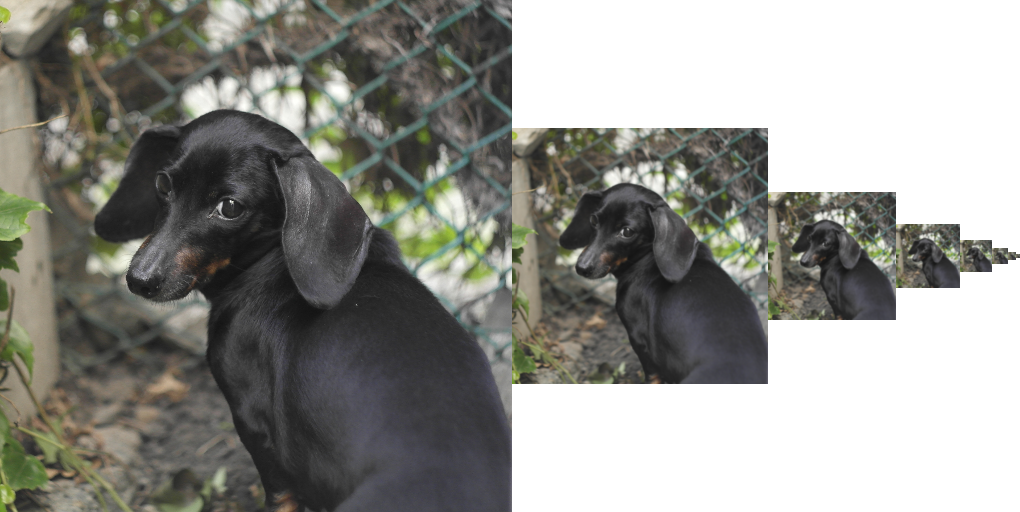
\includegraphics[width=7.65truecm, height=3.84truecm]{images/gauss_pyramid.png}
\caption{Gauss piramis}
\label{fig:gausspyramid}
\end{figure}

A módszer \textit{Spare Optical-Flow}-t valósít meg, vagyis egymástól különálló pontokat vizsgál, ellentétben a \textit{Dense Optical-Flow} módszerekkel, melyek a teljes kép vizsgálatával számolják ki az elmozdulás vektorokat. \cite{bradski2008learning} Az utóbbi módszerek számításigénye kifejezetten magas. Valós idejű alkalmazás esetén problémákba ütközhetünk gyengébb hardverek esetében. A mozgás valós idejű detektálására a \textit{Spare Optical-Flow} módszerek is kielégítő eredményekkel szolgálnak, néhány trükk alkalmazása mellett. Ilyenek például a már említett \textit{kép-piramisok} használata a gyors mozgások pontos követésére és a vizsgálandó pontok kijelölésének a stratégiája is. A pontok kijelöléséhez egy rácsszerkezet használatát gondoltam a legmegfelelőbbnek, ahol a pontok a rács metszéspontjaiban helyezkednek el. A képtartományt ily módon egyenletesen fedik le a pontok.

\Section{Rácspontok kezelése}

Az \textit{Optical-Flow} eljárást tetszőleges számú pontra elvégezhetjük. Ha létrehozhatunk egy rácsszerkezetet fix pontokkal, akkor a képtartományt egyenletesen lefedhetjük a pontok halmazával.
Ezen pontokat felhasználva minden iterációban az éppen aktuális és az egyel korábbi szürkeárnyalatos képkockákra elvégezhetjük az eljárást és így minden esetben kapunk egy új ponthalmazt, amely az eljárás eredménypontjait tartalmazza. Az eredeti és az új pontok párjaiból egy vektormezőt kapunk.

\begin{figure}[h]
\centering
\frame{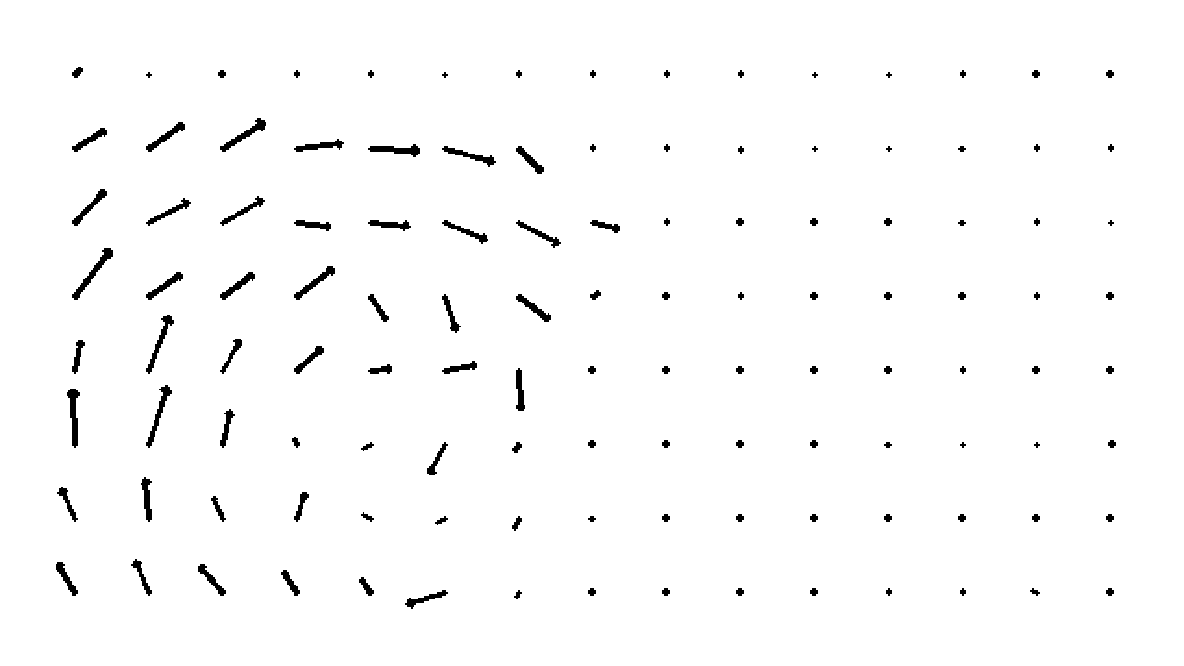
\includegraphics[width=11.2truecm, height=6.3truecm]{images/vectorField_screenshot.png}}
\caption{Képernyőfotó a vektormezőről}
\label{fig:vectorfield}
\end{figure}

A mozgás detektálása rácspontok segítségével kevesebb számítást igényel, mintha minden pixel elmozdulását vizsgálnánk és az elmozdulás becslésére is elfogadható eredményeket kapunk.
A rács sűrűségét tetszőlegesen megadhatjuk. Minél sűrűbb a rács szerkezete, annál több pontot vizsgál a szoftver, ami nagyobb pontosságot is eredményez. Viszont a sűrűbb rács használata a futási időt is befolyásolja. Egy gyengébb hardver esetén nem ajánlott magas sűrűség értékkel futatnunk a programot, mivel tapasztalataim szerint jelentős lassulásra számíthatunk.

A rácspontok helyzetének meghatározásához elsősorban definiálnunk kell egy sűrűségi változót. A sűrűség-értéknek kettő-hatványának kell lennie, hogy a négyzetes rácsszerkezet pontosan illeszkedjen a videófolyam képkockáira, amelyek képaránya általában 16:9-es vagy 4:3-as lehet. A videófolyam felbontása forrásonként változhat. Hasonló képarányok esetében minden esetben azonos mennyiségű pontot generálhatunk, ha a pontok közötti távolságot, vagyis a \textit{lépésközt}, a képkocka felbontásának és a rácssűrűségnek a függvényében határozzuk meg.
\begin{align*}
\textit{lépésköz} = \frac{\textit{szélesség}}{\textit{sűrűség}}
\end{align*}
, ahol a \textit{szélesség} a képkocka szélessége pixelekben mérve.\\
A \textit{lépésköz} érték segítségével határozhatjuk meg a pontok helyzetét.\\
\newline
\noindent \textbf{Rácspontok$\_$generálása}(szélesség, magasság, lépésköz, @rács)\\ 
\textbf{FOR} i $\leftarrow$ lépésköz \textbf{TO} (magasság/lépésköz)-1 \textbf{DO}\\
\indent \textbf{FOR} j $\leftarrow$ lépésköz \textbf{TO} (szélesség/lépésköz)-1 \textbf{DO}\\
\indent \indent rács $\leftarrow$ rács.append([j,i])\\
\textbf{RETURN} rács

\Section{Hőtérkép}

A vektormező egyes pontjait vizsgálva szerkeszthetünk egy ún. \textit{Hőtérkép}-et, amelyben különböző intenzitásértékekkel jelöljük az egyes vektorok hosszait. A \textit{Hőtérkép} egy $n \times m$-es mátrix, ahol $n$ a vektormező sorainak, $m$ pedig az oszlopainak a száma. A \textit{Hőtérkép} minden eleme egy BGR (blue, green, red) hármas értékkel van ellátva. Ezen értékek jelölik az egyes elemek színét.\\
Az értékek a következőképpen kerülnek kiszámításra:\\
\newline
\noindent \textbf{Hőtérkép$\_$kiszámítása}(@vektormező, érzékenység, @hőtérkép)\\ 
Input paraméter: vektormező (n$\times$m-es mátrix), érzékenység\\
Output paraméter: hőtérkép\\
\textbf{FOR} i $\leftarrow$ 1 \textbf{TO} Hossz(vektor$_n$) \textbf{DO}\\
\indent \textbf{FOR} j $\leftarrow$ 1 \textbf{TO} Hossz(vektor$_m$) \textbf{DO}\\
\indent \indent hőérték$_{ij}$ $\leftarrow$ hossz(vektor$_{ij}$)*érzékenység\\
\indent \indent \textbf{IF} hőérték$_{ij}$ > 255\\
\indent \indent \indent \textbf{THEN} hőérték$_{ij}$ $\leftarrow$ 255\\
\indent \indent hőtérkép$_{ij}$ $\leftarrow$ (255-hőérték$_{ij}$, 0, hőérték$_{ij}$)\\
\textbf{RETURN} hőtérkép\\
\newline
0 pixel hosszúság esetén az adott indexű elem (255, 0, 0) értéket kap, vagyis kék színnel jelöljük. Ha egy adott vektor számított hőértéke eléri a 255-öt, a hozzá tartozó \textit{hőtérkép-érték} (0, 0, 255) intenzitásértéket kap, vagyis tiszta piros színnel fog megjelenni.
A \textit{érzékenység} értékkel állíthatjuk be, hogy mely vektorhosszakat vegyen a program figyelembe. Az érték megadja, hogy milyen mértékű legyen a vektorok nagyítása, befolyásolva ezzel a számított \textit{hőértéket}.

\begin{figure}[h]
\centering
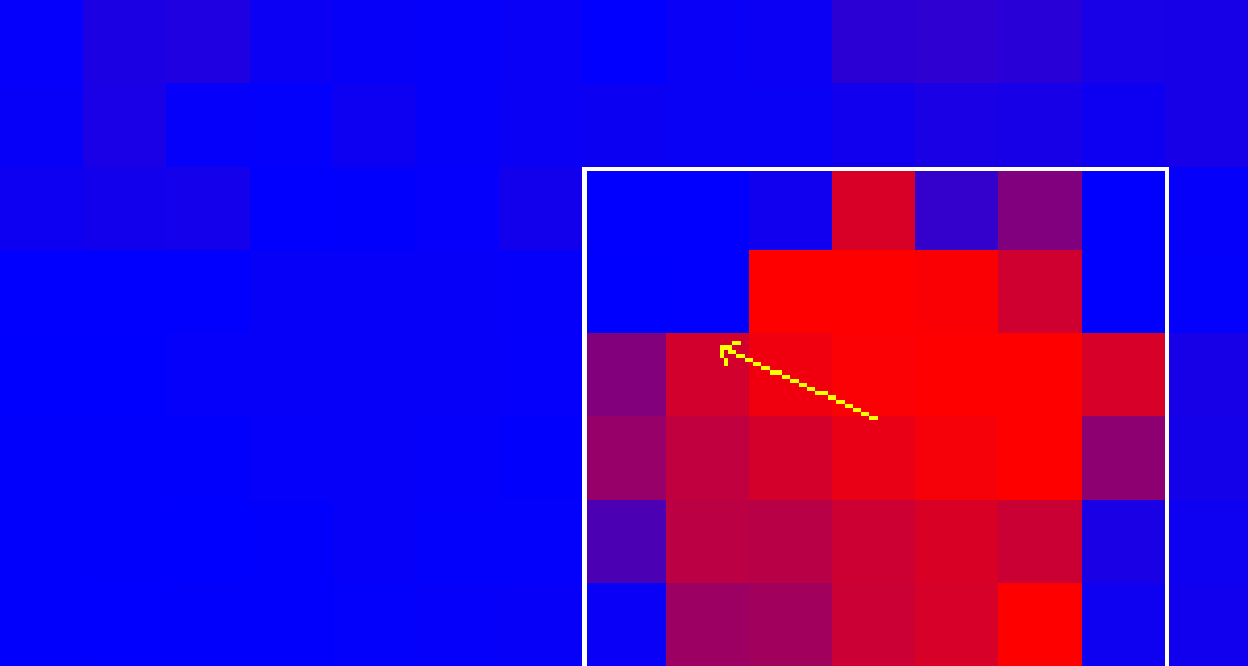
\includegraphics[width=11.2truecm, height=6.3truecm]{images/HeatMap_screenshot.png}
\caption{Képernyőfotó a hőtérképről}
\label{fig:heatmap}
\end{figure}

Az így kapott mátrixból ezután különféle információkat nyerhetünk ki. Az intenzitás értékeket vizsgálva meghatározhatjuk a nagyobb elmozdulások csoportjait. Ehhez küszöbölni kell a mátrixot, majd a kapott képen kontúrok keresésével meg lehet állapítani, hogy mely vektorok tartoznak egy csoportba. A csoportokat egy bizonyos intenzitás érték fölött érdemes keresni, vagyis az olyan vektorok összetartozó halmazai az érdekesek számunkra, amelyekben a vektorok hossza egy bizonyos határt elér. Az esetlegesen előforduló képzajok és az a videófolyamon megfigyelhető egyéb anomáliák miatt, amelyek a vektormező értékeire is hatással lehetnek, meg kell szabnunk a csoportok minimális területét. A megfelelően megválasztott értékek mellett a képzajból származó hibás értékek nem befolyásolják a program működését.
A \ref{fig:heatmap} ábrán megfigyelhető, hogy az összetartozó értékek fehér kerettel vannak jelölve. Továbbá a csoportok elmozdulásának irányai sárga nyilakkal vannak ábrázolva. A csoportokat külön-külön vizsgálva további értékes információkhoz juthatunk. Ilyen például az egyes csoportok iránya is, amelyet egy lokális eredővektor számításából kaphatunk meg. A csoportokat felhasználhatjuk további funkciók megvalósítására is, mint például a \textit{Többpontos kezelés}, a \textit{Rotation}, valamint az \textit{OCR-gesztus} vizsgálatára is.

\Section{Kontrollpontok és vektorok számítása}

\SubSection{Sweep}

A \textit{Sweep} gesztus két tulajdonsággal írható le: A mozgás irányával és hosszával. A mozgás irányát egy $\vec{v}\in\Bbb R^2$ irányvektorral határozhatunk meg, amelyet a \textit{vektormező} globális eredővektoraként kapunk meg.
\begin{align*}
  \vec{v} = \sum_{i=1}^n\vec{u_i}
\end{align*}
, ahol $\vec{u}$ a teljes képre vett vektormező vektorai.\\
A mozgás hossza a vektormező vektorainak átlagos hosszában mérhető és pixelszámban fejezhető ki.
\begin{align*}
  \overline{x}=\frac{\sum_{i=1}^n \left|\vec{v_i}\right|}{n}
\end{align*}
, ahol $n$ a vektormező vektorainak a száma.

\begin{figure}[h]
\centering
\frame{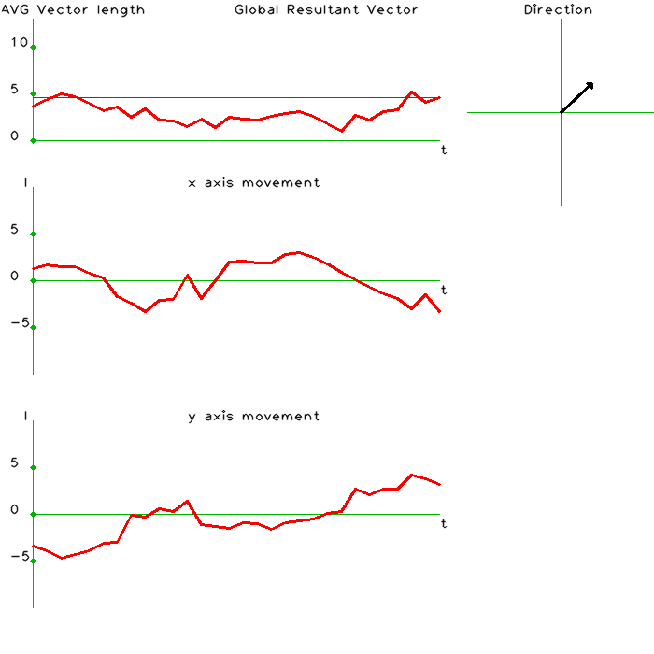
\includegraphics[width=11.86truecm, height=5truecm]{images/ResultantPlot_screenshot.png}}
\caption{Képernyőfotó a globális eredővektor grafikonjáról}
\label{fig:resultantplot}
\end{figure}

Az ábrán megfigyelhető a globális eredő vektor hosszainak változása egy 30 képkockás \textit{csúszóablakban} és az éppen aktuális irányvektor is.

\SubSection{Shift}

A \textit{Shift} tulajdonsággal rendelkező virtuális elemeknek mindig van egy aktuális pozíciójuk $(x,y)$, szélességük és hosszuk $(w,h)$, illetve sebesség értékük $v_{xy}$ a két tengelyre vonatkozóan.

A \textit{Shift} viselkedésének meghatározásához első lépésként az adott virtuális elem területére eső vektorokból $\vec{v}_l$  lokális eredővektort számolunk. Az elem területére eső vektorok és a lokális irányvektor meghatározható az elem pozíciója és a mérete alapján a következő módon:
\begin{align*}
  (i_1, j_1), (n, m) &= \lfloor \frac{(x,y),(w,h)}{\textit{rács lépésköze}} \rfloor\\
  \vec{v_l} &= \sum_{i=i_1}^n \sum_{j=j_1}^m \vec{u}_{ij}
\end{align*}
Az eredővektorból ezután irányvektort számolunk. Majd az irányvektor segítségével kiszámoljuk az elem sebességét:
\begin{align*}
  v_{xy} = v_{xy} + \frac{\vec{v}_l}{(n \cdot m)} \cdot \textit{gyorsulás}
\end{align*}
, ahol $\textit{gyorsulás} > 0$.\\
Az elem pozíciója $(x,y)$ a sebesség függvényében változik.
\begin{align*}
  (x,y) = (x,y)+v_{xy}
\end{align*}
A sebesség értéket minden iteráció végén tompítani kell, hogy a kezelt virtuális elem meg tudjon állni egy bizonyos ponton. Ha az adott elemet nem éri tovább erő, akkor a tompítás lassulást eredményez, a sebesség csökkenni fog. Olyan hatást is el tudunk érni egy helyesen megválasztott értékkel, mintha az eltolás után az elem csúszós felületen mozogna és így fokozatosan lassul le az iterációk során.
\begin{align*}
  v_{xy} = v_{xy} \cdot \textit{tompítás}
\end{align*}
, ahol $0 \leq \textit{tompítás} < 1$

% Ide még lehet jöhetne majd egy szemléltető képernyőkép, vagy valami ábra...

\SubSection{Drag}

A \textit{Drag} az elem elkapása utáni állapot jelenti, amikor a felhasználó az elkapott elem helyzetét szabadon változtathatja, majd új pozíciójára teheti. Ennek a funkciónak a megvalósításához többféleképpen is hozzáláthatunk.

Az első ötletem szerint a vektormező vektorait felhasználva lokális eredővektorokat számolva becsülte volna meg a program a mozgatandó virtuális elem új helyzetét. Ez a megoldás gyakorlatban az elvárásokat nem elégítette ki. Több probléma is adódott ezzel a megoldással. A \textit{Rács} lyukacsossága miatt nem mindig esett vizsgálandó pont a mozgás helyére. Az egyes kiugró értékek is befolyásolták a végeredményt, a mozgatandó elemek ilyen esetekben gyorsabban mozogtak a vártnál. Ez a megoldás tehát nem tűnt stabilnak, a vektormező rácsának sűrítésével pedig a program jelentős lassulásba ütközött volna. Más megoldás után kellett kutatni.

Mivel a \textit{Drag}-et előreláthatólag a prezentáló csak rövid időszakaszokban fogja használni, ezért a következő ötlettel áltam elő: a \textit{Blink} gesztus pozíciójára kontollpont(okat) illeszthetnénk, melyekre külön-külön elvégezhetnénk az \textit{Optical-Flow} eljárást és a pont vagy a pontok súlypontjának pozíciója függvényében változna a mozgatandó virtuális elem pozíciója is. Már egyetlen kontrollpont használata is kielégítő eredményt adott. Több kontrollpont használata csupán csak a biztonság érdekében tűnik megfelelőnek. Ha esetleg egy pont új pozícióját rosszul becsülné meg az eljárás és a pont egy bizonyos ponton leragadna, akkor maradjanak olyan "tartalék" pontok is, amelyek a funkció helyes működését biztosítani tudják.

\SubSection{Blink}

A \textit{Blink} gesztusok felismerésére elsősorban egy ún. \textit{Frame differencing} technikát kell alkalmaznunk.
Ehhez a videófolyam aktuális képkockájának és az egyel korábbi képkockájának abszolút különbségét kell meghatározni, majd az így kapott képen küszöbölést kell végrehajtani. Eredményképp egy olyan képet kapunk, amelyen az elmozdulás figyelhető meg fehér színnel jelölve. A keletkezett képen különféle alakzatok alakulhatnak ki. Az egyes mozdulatok hasonló nyomot hagynak maguk után. Így tehát egy \textit{Blink} mozdulat leadásakor jellegzetes mintázat rajzolódik ki.

\begin{figure}[h]
\centering

\includegraphics[width=5truecm, height=5truecm]{images/Grab_screenshot.png}
\caption{Egy Blink mozdulat pillanatképe}
\label{fig:blink}
\end{figure}

A \textit{Frame differencing} technika a teljes képtartományra vonatkozik, minden iterációban elvégezhetjük, hogy a videfolyamon történő mozgásról információkat kapjunk. A \ref{fig:blink} ábrán megfigyelhető, hogy nem csupán a legfrissebb két képkocka adatai vannak jelen a képen. Ezt a jelenséget egy keverési technikával érhetjük el. A korábbi mozdulatok rajzolatai alacsonyabb intenzitás értékekkel jelennek meg, míg a legfrissebb értékek 255 intenzitással vannak jelölve.

A gesztus detektálásához rögzített hosszúságú jellegvektorokra lesz szükségünk. A \textit{Frame differencing} technika képének dimenzió megegyeznek a videófolyam felbontásával. Így például 640$\times$480 felbontás mellett 307200 hosszúságú jellegvektorokat kapunk. A gesztus ily módon történő detektálása nem a legoptimálisabb megoldás. A \textit{Frame differencing} kép felbontásának csökkentésével pedig romolhat az információ minősége is.
A \textit{Blink} gesztusról feltételezhetjük, hogy a videófolyam egy kis területén fog jelentkezni. A vizsgálandó terület méretének, a jellegvektorok fix hosszai miatt, előre meghatározottnak kell lennie. A pontosabb becslés érdekében felhasználhatjuk a vektormező adatait is. A \textit{Blink} területére eső vektorok irányvektorait figyelve a mozgásról bővebb információt kapunk. Tapasztalati eredmények alapján a 16-os rácssűrűségű vektormezőn 5$\times$5-ös tartományon belül számíthatunk \textit{Blink} gesztus adataira. Mivel a \textit{Hőtérkép} segítségével meghatároztuk az összefüggő vektorok csoportjait, a csoport súlypontját tekinthetjük a \textit{Blink} gesztus középpontjának. Ezután a középpontot felhasználva meghatározandó az 5$\times$5-ös csoport a vektormező mátrixára nézve. A mátrix szélein és a sarkoknál, az indexelés helyessége miatt meg kell szabnunk, hogy a középpont minimum 2 lépés távolságra lehet a szélektől. Ha esetleg ez nem teljesülne, a legközelebbi helyes pontot jelöljük ki középpontnak. Ha sikeresen meghatároztuk a \textit{Blink}-re eső vektorok indexeit, a vektormező indexelt kezdőpontjainak értékeit felhasználva kiemelhetjük a \textit{Frame differencing} képből a \textit{Blink} gesztus tartományát. Az eredeti képből kivágott kép jóval kisebb lesz, a felesleges értékekből is kevesebb jelentkezik majd.
A kapott kép dimenzióit skálázással tovább csökkenthetjük egy bizonyos pontig, hogy a detektálás minél kevesebb memóriát vegyen igénybe. Szintén empirikus értékek szerint a gesztus képét egy 16$\times$16-os mátrixra csökkenthetjük. Ebben az esetben a jellegvektorok hossza 256-ra csökken. A vektormező értékeit is felhsználhatjuk a pontosabb detektálás érdekében. Mivel 5$\times$5-ös területet szabtunk meg, ez további 25 jellegvektort jelent. Érdemes irányvektorokat használni, így a gesztus a videófolyamon megfigyelhető helyzete nem befolyásolja a végeredményt.

\SubSection{Rotation}

A \textit{Rotation} gesztus két tulajdonsággal íható le: ezen gesztusnak mindig létezik egy elméleti középpontja, ami körül történik az elmozdulás, valamint van iránya is.
Becslést adni a mozgás lehetséges középpontjának pozíciójára a vektormező elemzésével célszerű.
A vektorokhoz egyenes egyenleteket szerkeszthetünk. Az egyenes egyenletének egy pontja a vektor kezdőpontja lesz, a normálvektora pedig az egyenes irányvektora.

\begin{figure}[h]
\centering
\frame{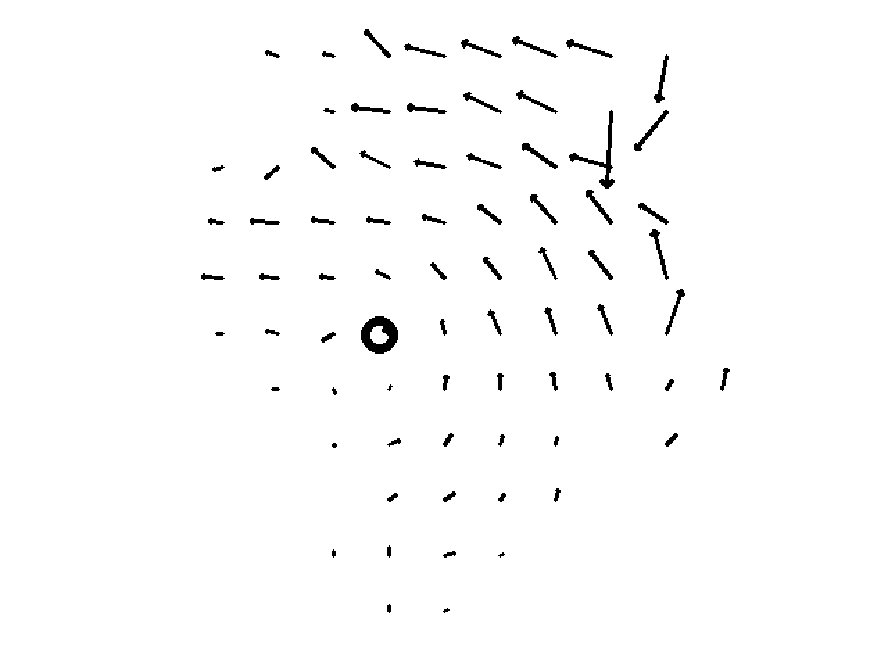
\includegraphics[width=8.88truecm, height=6.66truecm]{images/swirl_screenshot.png}}
\caption{A vektormező egy állapota a becsült forgási középponttal}
\label{fig:rotation}
\end{figure}

Két egyenletből álló egyenletrenszer megoldásaként megkapjuk az $x,y$ ismeretlen értékeket, melyek a két egyenes metszéspontjának a pozícióját adják meg.
A metszéspontokat számolva létrejön egy ponthalmaz, amelynek súlypontja az elméleti középpont közelében fog elhelyezkedni.
A programom \textbf{jelenleg} csupán a szomszédos vektorok egyenleteit oldja meg, ezzel számítási időt spórolva meg, kedvező futási időt biztosítva. A becslés pontossága viszont romlani fog.

Ha pedig több \textit{Rotation} pontot is vizsgálni szeretnénk, akkor segítségül hívhatjuk a \textit{Hőtérkép}-ből kinyert vektorcsoportok halmazait, majd ezen csoportokon külön-külön elvégezhetjük az eljárást a lokális súlypontok után kutatva.

\SubSection{Többpontos kezelés}

A \textit{Hőtérkép}-et vizsgálva azonosíthatunk és elkülöníthetünk vektorok halmazait egymástól. Az így kapott csoportokat vizsgálva további funkciókat valósíthatunk meg. A több ponttal irányítható funkciók közé tartozhatnak a \textit{Widget}-eken végrehajtható különféle manipulációk, mint például a skálázás is. További komplexebb gesztusok felismeréséhez is felhasználhatnánk a pontok egymáshoz képesti vizsgálatából kapott eredményeket.
Minden vektorcsoporthoz tartozik egy-egy lokális eredővektorból számított irányvektor, mely a vektorcsoport elmozdulásának irányát mutatja.
A skálázás műveletéhez két vektorcsoportot feltételezve az alábbi módon vizsgálhatjuk a két pont egymáshoz képesti elmozdulását.
Irányok esetében $\vec{u},\vec{v}\in \Bbb R^2$ esetén
\begin{align*}
\vmatrix \vec{u}+\vec{v} \endvmatrix &< \varepsilon_{\text{irány}}\\
&\approx \vec{0}
\end{align*}
Amennyiben a két pont iránya teljesen ellentétes, akkor a kapott érték a null vektorhoz közelít. Érdemes normalizált vektorokat használni, ha csupán az elmozdulás irányát szeretnénk vizsgálni és az egyes lokális irányvektorok hosszától el szeretnénk tekinteni.

\SubSection{OCR-Gesture}

A prezentáló személy bizonyos mozdulatokat elvégezve további funkciókat érhet el. Az ilyen gesztusok egy fajtája általában a magyarázó mozgástól eltérőek, bizonyos pályákat követnek. Ilyen mozdulatok lehetnek például egy kör, vagy egy L betű, vagy különféle minták rajzolása levegőbe. Az egyes mozdulatok hasonló mintázatot követnek.
Az ilyen típusú gesztusok felismeréséhez felhasználhatjuk az \textit{OCR}, vagyis az \textit{Optical Character recognition} (Optikai karakter felismerés) módszert is, mely írott karakterek felismerésére szolgál. 
Az OCR kipróbálásához rendelkezésre áll egy ingyenes adatkészlet is, a MNIST, amely 70.000 kisfelbontású képet tartalmaz írott számokról 0-9-ig. Segítségével különféle osztályozók taníthatók be, illetve az osztáyozók tejesítményének egyik mérőeszközévé vált az idők során. Az osztályozómodell betanításához a jellegvektorok értékeit a szürkeárnyalatosképek intenzitásértékei adják. Ha egy új osztályozó rendszert fejlesztenek, valószínűleg a MNIST adatkészlettel is kipróbálják azt. \cite{geron2019hands}

Mivel a probléma hasonlít az OCR-hez, hasonló megoldást alkalmazhatunk a levegőben leírt gesztusok felismeréséhez is. A mozdulat képét egy, a \textit{Hőtérképpel} megegyező vászonra rajzolja rá a program. A vászon mérete 16-os rácssűrűség mellett 11$\times$15-ös, vagyis megegyezik a \textit{Hőtérkép} dimenzióival. A vászon alapszíne fehér, vagyis 255 inenzitás értékekkel van ellátva. A gesztus képét a \textit{Hőtérkép} elemzésénel kinyert kontrollpontok rajzolják a vászonra: A vektorcsoportnak meghatározandó a súlypontja, mely a virtuális ecset hegyét jelenti. A súlypont elmozdulását a vásznon 0 intenzitásértékek követik, vagyis az elvégzett mozdulatok képei fekete színnel jelennek meg a vásznon. Mivel az egyes mozdulatok hasonló mintázatot követnek, a vásznon megjelenő képük is hasonló lesz.

\begin{figure}[h]
\centering
\frame{
\includegraphics[width=10truecm, height=7.33truecm]{images/OCR-Gesture.png}}
\caption{Egy levegőbe leírt kör mintázata a 11$\times$15-ös vásznon}
\label{fig:ocr-gesture}
\end{figure}

A vászon frissítése két módszerrel történik. Az elmozdulás értékek egy csúszóablakban helyezkednek el, amelyben maximum  30 érték kaphat helyet. Továbbá ha a \textit{Hőtérkép}-en nem figyelhető meg kontrollpont, az elmozdulás értékek törlése felgyorsul, míg a teljesen üres vásznot nem kapjuk.

A felismerés pillanatát feltételekhez kell kötnünk. A mozdulat rajzolatának végső formája akkor alakul ki, amikor a felhasználó befejezte az adott mozdulatot. Ilyen esetben a videófolyamon nem figyelhető meg további mozgás. Az időzítés egyik feltétele mindenképpen a mozgás hiányának kell lennie. Ez többféleképpen is megfigyelhető, vizsgálhatjuk a globális eredővektorunkat is, vagy a \textit{Hőtérkép} segítségével meghatározott csoportok számát is figyelembe vehetjük. Mivel a mintázat rajzolásához is a vektorok összetartozó csoportját használtuk fel, az időzítés egyik feltételének a vektorcsoportok hiányát szabhatjuk meg. Egy másik feltétel a rajzolat aktuális állapotára vonatkozhat. Figyelembe vehetjük a vonalhosszat is, vagyis egy bizonyos vonalhossz alatt nem végeznénk el az osztályozási becslést. Ezen két feltétel biztosítja, hogy az osztályozási művelet végrehajtása a megfelelő pillanatban történjen, elkerülve a felesleges számításokat, hibás becsléseket.
A mozdulat osztályozása utáni pillanatban a vásznat törölnünk kell, vagyis csupa 255 intenzitásértékkel kell ellátnunk, hogy a megszabott feltételek tovább ne teljesüljenek a további becsléseket elkerülve.

A modell betanításához képekre lesz szükségünk, amelyeket a programmal egyesével legyárthatunk és osztályozhatunk. További módszerek is léteznek a tanítóminta előállítására. Ilyenek lehetnek a minták generálása egy alap mintahalmazból zajosítással és egyéb megoldásokkal. Amint a minta rendelkezésünkre áll, a modell tanítható is. A témát egy másik fejezetben részletesen is kifejtem.
